\section{Progressive Hierarchical Refinement}
\label{phr}
\begin{figure}[H]
    \centering
    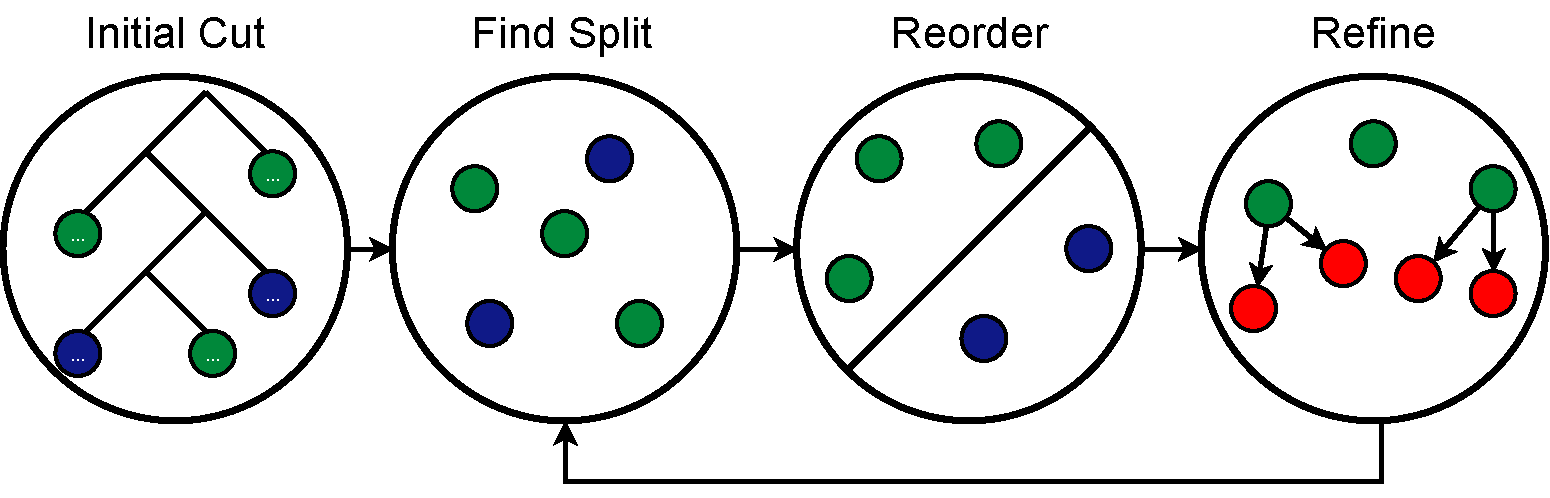
\includegraphics[width=400pt]{images/phr_algorithm.pdf}
    \caption{Illustration of the progressive hierarchical refinement algorithm.}
    \label{fig:phr}
\end{figure}
This section further explains the algorithm used to construct bounding volume hierarchies. Bounding volume hierarchies are constructed using progressive hierarchical refinement (PHR) as proposed by Hendrich et al.\cite{hendrich_parallel_2017}. As previously established, applying full sweep SAH to all scene primitives is magnitudes too slow. PHR tackles this problem by first constructing an auxiliary BVH, which then serves as a hierarchy to find much smaller sets of nodes on which full sweep SAH can be applied fairly inexpensively. The two resulting cuts are then refined, meaning that some nodes within those cuts are replaced by their children, if their bounding box surface area is above a certain threshold. Afterwards, the algorithm is applied recursively to the refined cuts until the full BVH is constructed. An illustration of that process can be seen in figure \ref{fig:phr}.

\subsection{Auxiliary Bounding Volume Hierarchy}
\label{aux}
As the auxiliary BVH is only needed as a description of the scene's hierarchy, construction speed is the main priority. Multiple fast builders have been tested in the original paper\cite{hendrich_parallel_2017}, but linear bounding volume hierarchies (\acrshort{lbvh}) turned out to be the best choice. LBVH was first proposed by Lauterbach et al.\cite{lauterbach09lbvh} as a top-down algorithm that assigns Morton codes to all primitives and then builds the tree as a binary radix tree. The algorithm itself has since been improved multiple times\cite{karras12lbvh,apetrei14lbvh,chitalu20lbvh} making it one of the fastest approaches to date\cite{meister21survey}. However, these approaches exploit the massive parallelism GPUs can provide by building the BVH in a bottom up fashion, which makes less sense on the limited amount of cores CPUs provide. Consequently, the approach used here is closer to the top-down algorithm proposed by Lauterbach et al.\cite{lauterbach09lbvh} with a few adjustments. 
\begin{figure}[H]
    \centering
    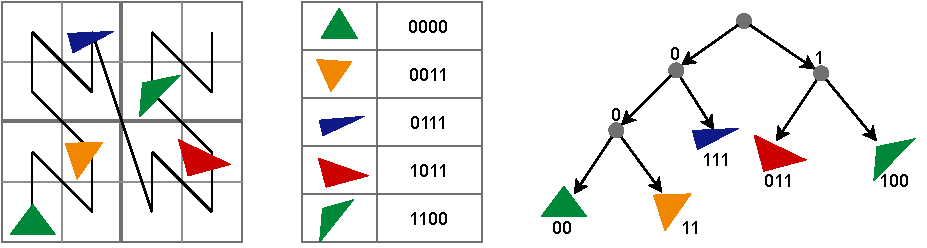
\includegraphics[width=400pt]{images/morton_curve.pdf}
    \caption{Left shows 2D Morton curve using 2 bits per dimension. The table in the center shows the corresponding Morton codes and the right shows the resulting tree structure, equivalent to a binary radix tree.}
    \label{fig:morton}
\end{figure}
Construction of the auxiliary BVH starts off by sorting all primitives along a Morton curve\cite{morton66curve}. This space filling curve subdivides the scene space into a uniform grid, resulting in Morton codes of fixed length (figure \ref{fig:morton}). Computation of Morton codes is done fairly efficiently by interleaving successive bits of the primitives' quantized bounding box centroids.

Morton codes are assigned in parallel by processing $[n/t]$ primitives per thread, with $n$ being the number of scene primitives and $t$ being the number of threads. Afterwards, the primitives are sorted according to their Morton code using a parallel bucket sort implementation. In each thread, $k=2^{12}$ empty buckets are created and filled with $[n/t]$ primitives. By using individual buckets for each thread, no further synchronization necessary for the bucketing. However, an atomic counter is used to keep track of the total number of primitives in each bucket across all threads, which is then used to find the intervals in the original array each bucket occupies. After bucketing is finished, all non-empty buckets with the same index are merged and directly written to the mentioned interval in the input array, before being sorted in place using Go's built-in sort function. This step is also done in parallel by utilizing the worker pattern to send buckets with the same index to each thread until all buckets have been processed.

The corresponding BVH can be constructed by recursively splitting the set of primitives at the highest bit within the current interval. This is done using a Go channel and entries representing a node in the finished tree. Each thread fetches such a node and finds the split in the corresponding array by applying linear search. If the node does not become a leaf, the resulting cuts are sent to the channel to be processed by idle threads.

Finally, the bounding boxes of the tree are updated in parallel by starting at the tree's leaves and traversing towards the root. Whenever a thread visits a node, the bounding box is updated using the child or primitive bounding boxes. Then the parents atomic counter is incremented and if all children are set, the thread also processes the parent. Otherwise, the thread fetches an unprocessed leaf from a queue. The same procedure is executed when refitting the LBVH on scene changes. 
\subsection{Algorithm}
\label{phr_algorithm}
The main progressive hierarchical refinement algorithm starts by identifying a set of nodes that separate root and leaves of the auxiliary LBVH. Nodes are selected in parallel using a priority queue. A thread pops an entry from that queue and compares its bounding volume surface area to a given threshold. If the surface area is below that threshold or the cut has reached its maximum size, the node is added to the initial cut. Otherwise, its children are inserted into the priority queue to be processed by another thread. The resulting cut is several magnitudes below the full primitive count and can be processed fairly inexpensively using full sweep SAH.

Cuts are split by evaluating an adapted version of the surface area heuristic for all three axis and choosing the split with the lowest cost. The cut becomes a leaf, if the cost of not splitting at all is the lowest. Each axis is evaluated by sorting nodes along given axis according to their bounding box centroid. The SAH cost for a split at the index $i$ in the sorted set is given as 
\[C(i)=S_L(i)n_L(i)+S_R(i)n_R(i)\]
where $S_L(i)$ and $S_R(i)$ are the bounding boxes surface areas of the left and right subsets and $n_L(i)$ and $n_R(i)$ are the number of nodes in the corresponding subtrees. Note that this expression is very similar to the SAH cost presented in section \ref{acceleration_structure_basics}. However, instead of using the number of primitives in the left and right cuts, the number of nodes is used. According to Hendrich et al.\cite{hendrich_parallel_2017}, this improves the performance by a few percent, as the number of nodes better reflects the complexity of the given subtree.

The SAH evaluation algorithm first computes all right costs $S_R(i)n_R(i)$ by incrementally extending the split bounding box and storing the partial costs, which is more efficient than computing the full bounding box at each step. The full cost is then calculated in the same fashion, extending the bounding box from the left to solve $S_L(i)n_L(i)$. 

Splitting the cut reduces the number of nodes in each new cut and doing so multiple times would lead to a cut size of one. To keep cuts at a larger size for longer and to better utilize the hierarchical information the auxiliary BVH can provide, cuts are refined after splitting. Keeping cuts at a constant size, as proposed by Hunt et al.\cite{hunt07lazybuild}, would become rather expensive towards the bottom of the tree due to the growing number of cuts. As a solution, Hendrich et al.\cite{hendrich_parallel_2017} proposed an adaptive refinement approach based on the current depth in the tree. This approach makes cuts shrink towards the bottom of the tree, which balances the computational cost between different levels of the tree. The BVH quality is not worsened significantly by doing so, as the impact of SAH gets lower further down the tree. 

Refinement works by comparing node bounding box surface areas to an adaptive threshold. Nodes with a surface area below this threshold are kept within the cut. Otherwise, the node is replaced by its children. This adaptive threshold is given as 
\[t_d = S /{2^{\alpha d + \delta}}\]
with $S$ being the surface are of the scene bounding box and $d$ the current depth in the tree. The parameter $\alpha$ describes how quickly cuts shrink towards the bottom and $\delta$ determines the size of the initial cut for $d=0$. The setting of these parameters determines the build-trace trade-off of the algorithm and is elaborated further in section \nameref{parameters}.

Construction of the BVH uses a similar setup as previously mentioned for the LBVH generation. A thread pool of $t$ threads pops entries from a channel, consisting of a cut and parent node index. The cut is split using the described method, the resulting cuts are refined and then fed back into the channel if the node did not become a leaf. Additionally, a higher branching factor can be specified to build a multi-BVH\cite{wald08multibvh}. In that case, a thread keeps splitting the biggest resulting cut until enough children have been generated or no more splits exist. The effect of multi-BVHs on the rendering performance is evaluated in section \ref{multi_bvh}.

\begin{figure}[H]
    \centering
    \subcaptionbox{Render}{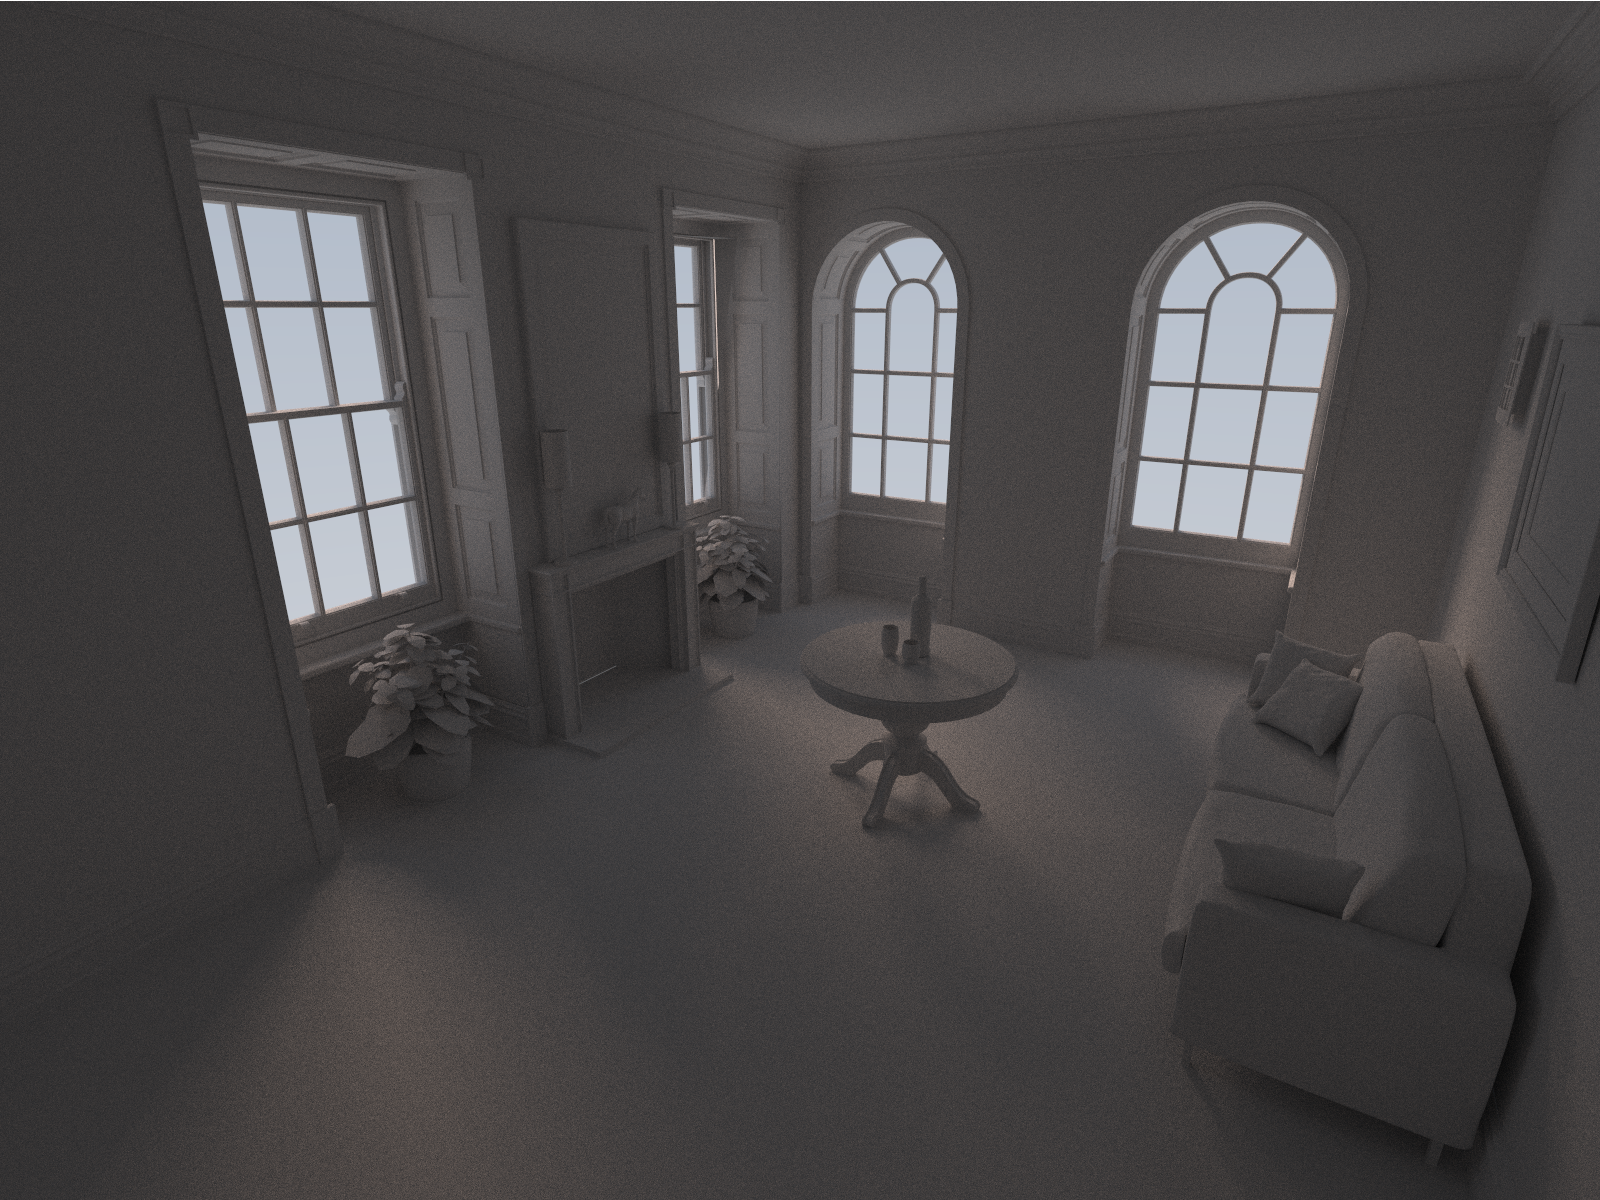
\includegraphics[width=0.3\textwidth]{images/fireplace_render.png}}
    \hfill
    \subcaptionbox{LBVH}{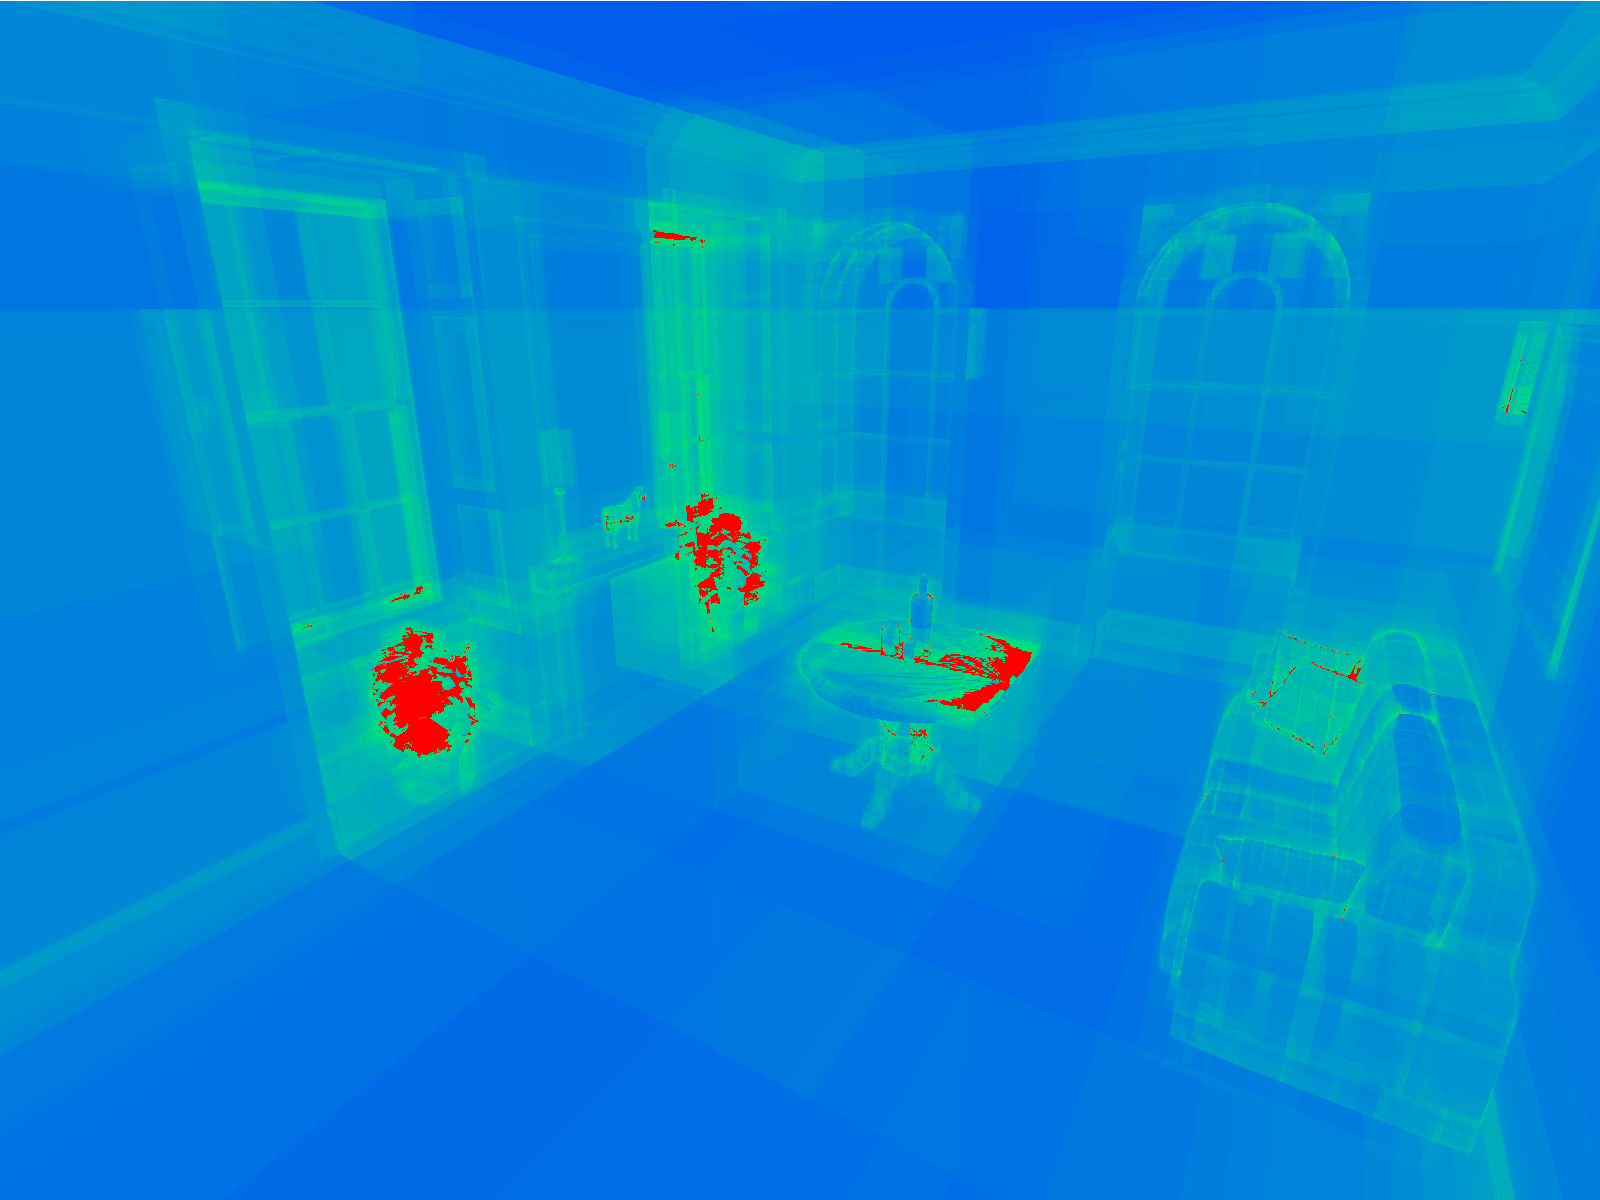
\includegraphics[width=0.3\textwidth]{images/fireplace_lbvh.png}}
    \hfill
    \subcaptionbox{PHR-HQ}{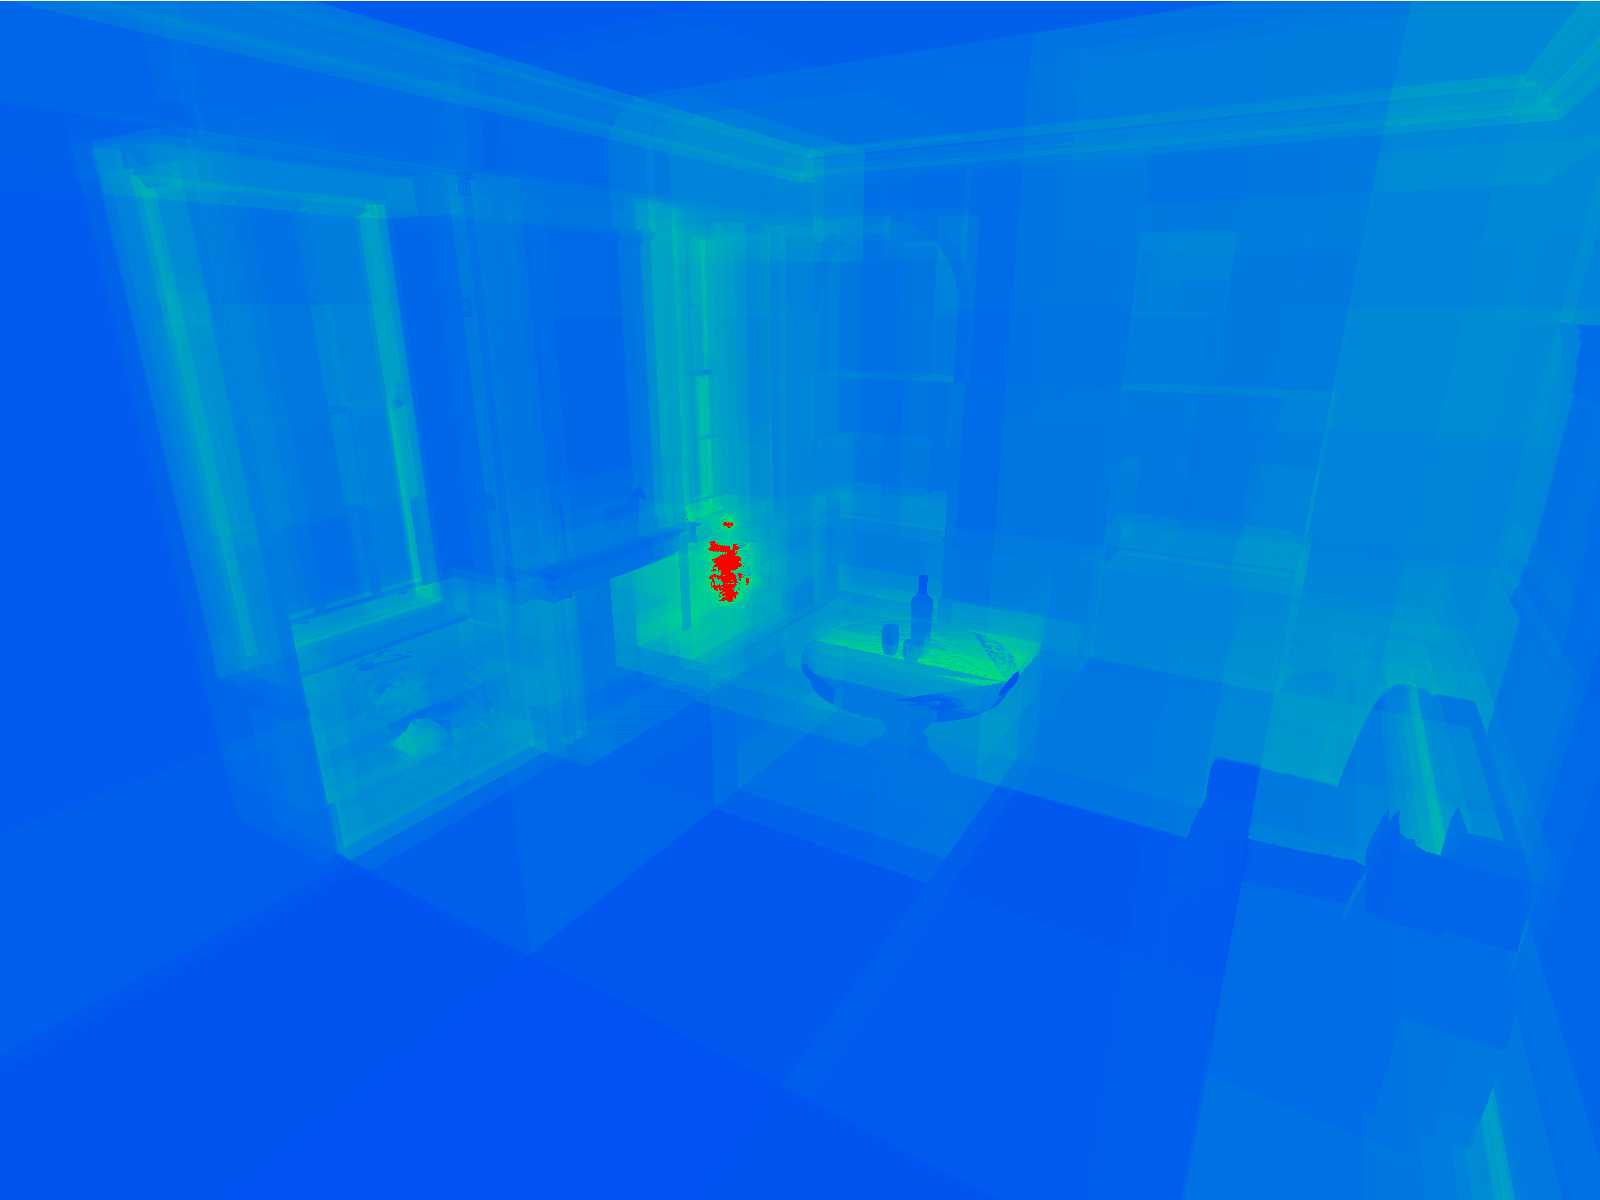
\includegraphics[width=0.3\textwidth]{images/fireplace_phr.png}}
    \caption{Visualization of the number of traversal steps for primary rays using LBVH and PHR (red color corresponds to 100 traversal steps per ray).}
    \label{fig:noise}
\end{figure}
\subsection{Integration into Interactive Path Tracing}
\label{phr_in_interactive}
An approach for integrating progressive hierarchical refinement into interactive applications was mentioned in the original paper\cite{hendrich_parallel_2017}, but its validation remained an open topic. The idea was to only build the auxiliary BVH once in the beginning and then refit it very efficiently between frames. Refitting is done by updating bounding boxes of all BVH nodes. The hierarchy of the structure stays unchanged during this procedure. As described in the end of section \ref{aux}, this is done using a parallel recursive procedure that traverses the tree in a bottom-up fashion and merges child bounding boxes using an atomic counter for synchronization. Doing so is fairly efficient in comparison to a full BVH rebuild, however, refitting generally leads to some extend of BVH quality loss, especially for significant scene changes. Applying PHR to the refitted tree counteracts this loss by building a new BVH.
\cleardoublepage